\documentclass[border=4pt]{standalone}\usepackage[utf8]{inputenc}\usepackage[T1]{fontenc}\usepackage{mathptmx}
\usepackage{tikz}
\usetikzlibrary{arrows.meta,positioning,calc,fit,backgrounds}
\tikzset{>={Stealth[length=2.2mm]}, font=\small,
 blk/.style={draw, line width=0.8pt, fill=white, align=center, inner sep=3pt, text width=#1, minimum height=1.1cm},
 blk/.default=3.0cm,
 iut/.style={fill=black!14},
 ext/.style={draw, dashed, line width=0.5pt, align=center, inner sep=3pt, text width=#1, minimum height=1.0cm, fill=white},
 ext/.default=2.6cm,
 grp/.style={draw=black!55, dashed, line width=0.5pt, fill=black!4, inner sep=7pt},
 glab/.style={font=\small\itshape, text=black!75, anchor=north west, inner sep=2pt},
 lab/.style={font=\footnotesize, inner sep=1.5pt, fill=white},
 pw/.style={line width=2.2pt, -{Stealth[length=2.6mm]}},
 dg/.style={line width=0.6pt},
 an/.style={line width=0.8pt, dashed},
 rf/.style={double, double distance=1.2pt, line width=0.4pt},
 cd/.style={line width=0.6pt, dotted}}

\begin{document}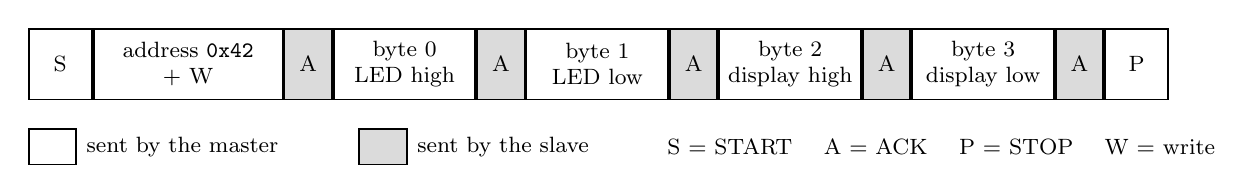
\begin{tikzpicture}[f/.style={draw, line width=0.7pt, minimum height=0.9cm, align=center, font=\footnotesize, inner sep=2pt}]
\def\x{0}
\node[f, minimum width=0.8cm, anchor=west] (s) at (0,0) {S};
\node[f, minimum width=2.4cm, anchor=west] (ad) at (s.east) {address \texttt{0x42}\\+ W};
\node[f, fill=black!14, minimum width=0.6cm, anchor=west] (a0) at (ad.east) {A};
\node[f, minimum width=1.8cm, anchor=west] (b0) at (a0.east) {byte 0\\LED high};
\node[f, fill=black!14, minimum width=0.6cm, anchor=west] (a1) at (b0.east) {A};
\node[f, minimum width=1.8cm, anchor=west] (b1) at (a1.east) {byte 1\\LED low};
\node[f, fill=black!14, minimum width=0.6cm, anchor=west] (a2) at (b1.east) {A};
\node[f, minimum width=1.8cm, anchor=west] (b2) at (a2.east) {byte 2\\display high};
\node[f, fill=black!14, minimum width=0.6cm, anchor=west] (a3) at (b2.east) {A};
\node[f, minimum width=1.8cm, anchor=west] (b3) at (a3.east) {byte 3\\display low};
\node[f, fill=black!14, minimum width=0.6cm, anchor=west] (a4) at (b3.east) {A};
\node[f, minimum width=0.8cm, anchor=west] (p) at (a4.east) {P};
% legend
\node[f, minimum width=0.6cm, minimum height=0.45cm, anchor=west] (k1) at (0,-1.05) {};
\node[font=\footnotesize, anchor=west] at (k1.east) {sent by the master};
\node[f, fill=black!14, minimum width=0.6cm, minimum height=0.45cm, anchor=west] (k2) at (4.2,-1.05) {};
\node[font=\footnotesize, anchor=west] at (k2.east) {sent by the slave};
\node[font=\footnotesize, anchor=west] at (8.0,-1.05) {S = START \quad A = ACK \quad P = STOP \quad W = write};
\end{tikzpicture}\end{document}
